\documentclass[11pt]{beamer}


\usepackage{amssymb, amsmath, graphicx, caption, enumerate}
\graphicspath{ {images/} }
\usepackage{amsthm}
\usepackage{xargs}
\usepackage{scalerel}




\newcommand{\N}{\mathbb{N}}
\newcommand{\Z}{\mathbb{Z}}
\newcommand{\R}{\mathbb{R}}
\newcommand{\K}{\mathbb{K}}
\newcommand{\C}{\mathbb{C}}
\newcommand{\D}{\mathcal{D}}
\newcommand{\A}{\mathcal{A}}
\newcommand{\ds}{\displaystyle}
\newcommand{\op}[1]{\left(#1\right)}
\newcommand{\cp}[1]{\left[#1\right]}
\newcommand{\av}[1]{\left| #1\right|}
\newcommand{\st}[1]{\left\{#1\right\}}


\usepackage[colorinlistoftodos,prependcaption,textsize=tiny]{todonotes}
\newcommandx{\question}[2][1=]{\todo[linecolor=red,backgroundcolor=red!25,bordercolor=red,#1]{#2}}
\newcommandx{\change}[2][1=]{\todo[linecolor=blue,backgroundcolor=blue!25,bordercolor=blue,#1]{#2}}
\newcommandx{\add}[2][1=]{\todo[linecolor=OliveGreen,backgroundcolor=OliveGreen!25,bordercolor=OliveGreen,#1]{#2}}
\newcommandx{\improve}[2][1=]{\todo[linecolor=Plum,backgroundcolor=Plum!25,bordercolor=Plum,#1]{#2}}
\newcommandx{\thiswillnotshow}[2][1=]{\todo[disable,#1]{#2}}
\newcommandx{\remove}[2][1=]{\todo[linecolor=yelllow,backgroundcolor=yellow!10,bordercolor=red,#1]{#2}}


\newcommand\reallywidehat[1]{\arraycolsep=0pt\relax%
\begin{array}{c}
\stretchto{
  \scaleto{
    \scalerel*[\widthof{\ensuremath{#1}}]{\kern-.5pt\bigwedge\kern-.5pt}
    {\rule[-\textheight/2]{1ex}{\textheight}} %WIDTH-LIMITED BIG WEDGE
  }{\textheight} % 
}{0.5ex}\\           % THIS SQUEEZES THE WEDGE TO 0.5ex HEIGHT
#1\\                 % THIS STACKS THE WEDGE ATOP THE ARGUMENT
\rule{-1ex}{0ex}
\end{array}
}


\usetheme{CUDenver}
\renewcommand{\familydefault}{\sfdefault}
\usefonttheme[onlymath]{serif}
\usepackage{tikz}
\usetikzlibrary{arrows}
\setbeamertemplate{itemize items}{>>}
\setbeamertemplate{itemize subitem}[square]
\setbeamertemplate{itemize subsubitem}[ball]
\newcommand{\norm}[1]{\left\lVert#1\right\rVert}



\author{Jordan R. Hall}

\title[CUDenver Theme]{Active Subspaces via Monte Carlo Sampling}

\institute[UCD]{
Department of Mathematical and Statistical Sciences\\
University of Colorado Denver
}

\date{Monday, December 3, 2018}

\begin{document}
% ------------------------------------------------


\begin{frame}[t,plain]
    \titlepage
\end{frame}

% start the content of the presentation

\begin{frame}{Overview}


\tableofcontents
\end{frame}



% ------------------------------------------------
\section{Dimension Reduction and the Active Subspace}
% ------------------------------------------------

\begin{frame}

\begin{itemize}

	\item We consider functions $f: \Lambda \to \mathcal{D}$ where $\dim(\Lambda)=N$ is large and $\dim(\mathcal{D})=M$ is such that $M<N$ or $M<<N$.

\begin{itemize}
		\item Functions of interest may represent postprocessed quantities from the solution of complex physical models.
\end{itemize}

\item It is not often that every parameter has equal impact on function values -- usually some parameters matter more than others.

\item The dimension reduction techniques considered seek to explain outputs $f(\Lambda)$ in an \textit{active subspace} $\mathcal{A} \subset \Lambda$ for which $\dim(\A)<N.$

\begin{itemize}
\item A lower-dimensional representation of $f$ can save computational costs.

\end{itemize}


\end{itemize}


\end{frame}



\begin{frame}

\begin{itemize}

\item $\nabla f(\lambda)\in \Lambda$ is a column vector with rows containing the $N$ partial derivatives of $f$, which for this discussion we assume exist, and are square integrable in $\Lambda$ equipped with some probability density that is positive everywhere in $\Lambda$ and 0 otherwise.

\begin{itemize}
		\item We consider $\pi_\Lambda^\text{prior}(\lambda)$, the density describing our prior state of knowledge, which we abbreviate as $\pi_\Lambda$.
\end{itemize}

\item One transforms inputs $\lambda$ to the origin with some fixed variance, typically so that $\lambda\in [-1,1]^N$. We define

\end{itemize}

\begin{block}{Covariance in Gradient Space \footnotemark[1]}

\begin{equation} \label{eq:1}
W=\int_\Lambda \nabla f(\lambda) \nabla f(\lambda)^\top  \pi_\Lambda(\lambda) d\lambda,
\end{equation} 

\noindent which is an $N\times N$ symmetric positive semi-definite matrix.

\end{block}

%\footnotetext[1]{Constantine, Eftekkari, Wakin}
\footnotetext[1]{Constantine}


\end{frame}

\begin{frame}

\begin{itemize}



\item Interpreting $W$ as a certain covariance structure over $\Lambda$ leads one to the idea of computing the Singular Value Decomposition of $W$,

\begin{block}{Singular Value Decomposition (SVD) of $W$}

\begin{equation} \label{eq:2}
W=U\Sigma V^*,
\end{equation} 


\noindent where $U$ is $N \times N$ unitary, $\Sigma$ is $N \times N$ diagonal with the singular values of $W$ along its diagonal, and $V^*$ is $N \times N$ unitary.

\end{block}

\item We plot the singular values, $\{\sigma_i\}_{i=1}^n$ and seek a drop-off in magnitude between some pair of singular values, $\sigma_{j}$ and $\sigma_{j+1}$. The active subspace is the span of $u_1,\ldots,u_{j}$, which are the first $j$ columns of $U$, the left singular vectors of $W$. 


\end{itemize}

\end{frame}

\begin{frame}

\begin{itemize}

	\item For a point $\lambda \in \Lambda$, we define

\begin{block}{Projection into $\mathcal{A}$, \textit{active variables}}

\begin{equation} \label{eq:3}
  \mathcal{P}_\A(\lambda)=\sum_{i=1}^{j}\left( u_i^T \lambda\right)u_i \in \A, 
\end{equation}

\noindent which is the projection of $\lambda$ in the active directions of $f$.

\end{block}

\item We have arrived at the property that 

\begin{block}{Resolution of $f$ in $\mathcal{A}$}

\begin{equation} \label{eq:7}
f\left(\mathcal{P}_\A(\lambda)\right) \approx f(\lambda).
\end{equation}

\end{block}

\end{itemize}



\end{frame}

% ------------------------------------------------
\section{Active Subspaces via Monte Carlo}
% ------------------------------------------------


\begin{frame}

\begin{itemize}

\item Finding an active subspace requires forming an approximation to $W$ via Monte Carlo. Here we consider techniques in \footnotemark[1] \footnotemark[2].



\item We let $D_S=\{(\lambda_i,f(\lambda_i))\}_{i=1}^S$, which is a set of $S$ pairs of samples $\lambda_i \in \Lambda$ and their function values. One may use $D_S$ to approximate $\nabla f$. We denote each estimation to $\nabla f(\lambda_i)$ with $\reallywidehat{\nabla f}(\lambda_i)$.

\item We form the $N \times S$ matrix $\tilde{W}$ (which we present as $\tilde{W}^\top$)

\end{itemize}

\begin{block}{Monte Carlo Approximation to $W$ \footnotemark[1]}


\begin{equation} \label{eq:4}
\tilde{W}^\top:=\begin{bmatrix}
\reallywidehat{\nabla f}(\lambda_1)
\cdot \cdot \cdot
\reallywidehat{\nabla f}(\lambda_S)\\
\end{bmatrix}.
\end{equation}  

\end{block}

\footnotetext[1]{Russi, T.M.}
\footnotetext[2]{Constantine, Eftekkari, Wakin}

\end{frame}

\begin{frame}

\begin{itemize}

	\item Forming the SVD of $\tilde{W}$, $\tilde{W}=\tilde{U}\tilde{\Sigma}\tilde{V}^*$, we search for a drop off in the magnitude of the singular values $\{\tilde{\sigma}_i\}_{i=1}^S$. Assuming such a drop off occurs for an index $j:1<j<S$, we have the $j$ corresponding left singular vectors,$ \tilde{u},\ldots,\tilde{u}_{j}$.  
	
	\item Then we define

	\begin{block}{Monte Carlo approximation to $\A$}
	
	
	$$\A\left(f; D_S \right):=\text{span}\{\tilde{u},\ldots,\tilde{u}_{j}\},$$ the active subspace of $f$ with respect to the samples $D_S$.
	
	\end{block}		

	\item We check the extent to which the active subspace accounts for functions values $f(\lambda)$ 
by checking for resolution in a \emph{sufficient summary plot}, where we plot active variables against function values.


\end{itemize}



\end{frame}



% ------------------------------------------------
\subsection{Quick Example!}
% ------------------------------------------------

\begin{frame}

 \textbf{Example 1.} Let $\Lambda=[-1,1]^{11}$ and define $$f(\lambda)=\sum_{i=0}^{10} 2^{(-1)^i i}\lambda_i^2+\epsilon(\lambda),$$ where $\epsilon(\lambda)$ is a draw of additive noise corresponding to the input $\lambda$; here, we take draws of $\epsilon$ of order $10^{-4}$. We see that $\mathcal{D}=[0,2^{10}]$ and $N=11$, $M=1$. Note that the minimimum of $f$ is given by $0 \in \Lambda$. Here, as $i$ increases, terms in $f$ become either more important or less important, depending on whether $i$ is even or odd.


\end{frame}

\begin{frame}

\begin{center}

 
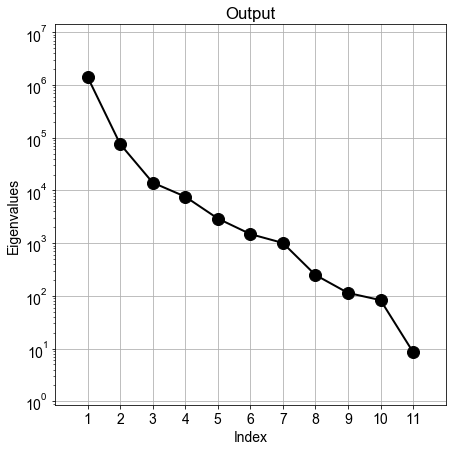
\includegraphics[scale=0.3]{eigs.png} 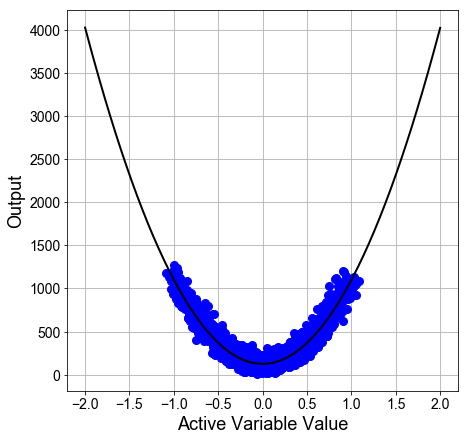
\includegraphics[scale=0.3]{surr.png}

Left: A plot of the eigenvalues of the matrix $\hat{W}$ formed from 1000 Monte Carlo samples in $\Lambda$. We see one dominant eigenvalue on the order of $10^6$. Right: A sufficient summary plot where all 1000 samples are projected into $\A$ and plotted against their function values; a quadratic surrogate fits the projected data with $R^2\approx 0.9$.

\end{center}



\end{frame}

\begin{frame}

\begin{center}

 
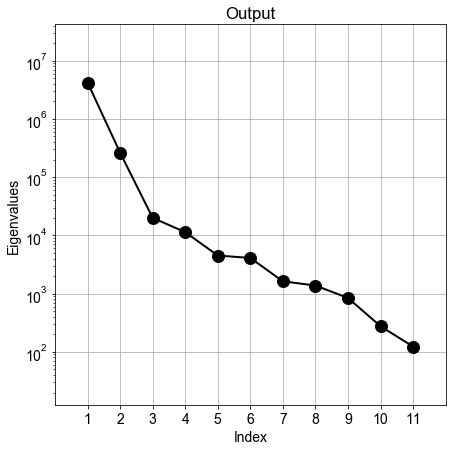
\includegraphics[scale=0.3]{DFO_eigs.png} 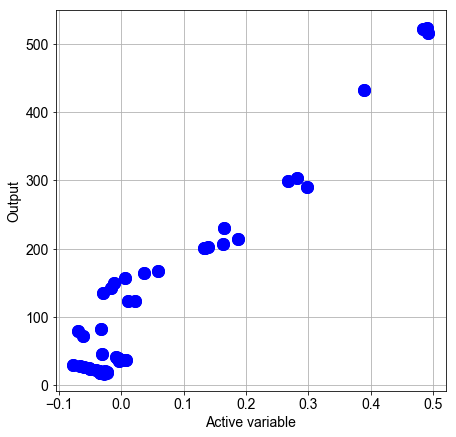
\includegraphics[scale=0.3]{DFO_suffsum.png}

Left: A plot of the eigenvalues of the matrix $\hat{W}$ formed from using 100 DFO iterates as samples in $\Lambda$. We again see one dominant eigenvalue between orders $10^6$ and $10^7$. Right: A sufficient summary plot where all 100 samples are projected into $\A$ and plotted against their function values.

\end{center}



\end{frame}


% ------------------------------------------------

\section{References}
% ------------------------------------------------
\begin{frame}[allowframebreaks]

%%%%%%%%%%%%%% References %%%%%%%%%%%%%%%%%%%%%%%%%
\begin{thebibliography}{65}

\bibitem{Constantine2015} Constantine, Paul G. ``Active Subspaces: Emerging Ideas for Dimension Reduction in Parameter Studies." SIAM, 2015.

\bibitem{ConstantineMC} Constantine, Eftekhari, Wakin. ``Computing Active Subspaces Efficiently with Gradient Sketching." Conference paper, 2015 IEEE 6th International Workshop on Computational Advances in Multi-Sensor Adaptive Processing (CAMSAP).


\bibitem{Russi} Russi, Trent M. ``Uncertainty Quantification with Experimental Data and Complex System Models." Dissertation, University of California Berkeley. 2010.




\end{thebibliography}






\end{frame}







\end{document}

